%%%%%%%% ICML 2020 EXAMPLE LATEX SUBMISSION FILE %%%%%%%%%%%%%%%%%

\documentclass{article}

% Recommended, but optional, packages for figures and better typesetting:
\usepackage{microtype}
\usepackage{graphicx}
\usepackage{subfigure}
\usepackage{booktabs} % for professional tables

% hyperref makes hyperlinks in the resulting PDF.
% If your build breaks (sometimes temporarily if a hyperlink spans a page)
% please comment out the following usepackage line and replace
% \usepackage{icml2020} with \usepackage[nohyperref]{icml2020} above.
\usepackage{hyperref}

% Attempt to make hyperref and algorithmic work together better:
\newcommand{\theHalgorithm}{\arabic{algorithm}}

% Use the following line for the initial blind version submitted for review:
\usepackage{icml2020}

% If accepted, instead use the following line for the camera-ready submission:
%\usepackage[accepted]{icml2020}

% The \icmltitle you define below is probably too long as a header.
% Therefore, a short form for the running title is supplied here:
\icmltitlerunning{Ordinal tensor denoising and completion}
\usepackage{wrapfig}
\usepackage{multirow}
\usepackage{graphicx}
%\usepackage[utf8]{inputenc} % allow utf-8 input
%\usepackage[T1]{fontenc}    % use 8-bit T1 fonts
\usepackage{hyperref}       % hyperlinks
\usepackage{url}            % simple URL typesetting
%\usepackage{booktabs}       % professional-quality tables
\usepackage{amsmath,amssymb}
\usepackage{amsthm}    % blackboard math symbols
%\usepackage{nicefrac}       % compact symbols for 1/2, etc.
%\usepackage{microtype}      % microtypography
\usepackage{bm}
%\usepackage{subfig}
%\usepackage[english]{babel}
%\usepackage{algorithm}
%\usepackage{appendix}
\usepackage{mathtools}
\mathtoolsset{showonlyrefs}
\usepackage{enumitem}
\theoremstyle{plain}
\newtheorem{thm}{Theorem}[section]
\newtheorem{lem}{Lemma}
\newtheorem{prop}{Proposition}
\newtheorem{pro}{Property}
\newtheorem{assumption}{Assumption}

\theoremstyle{definition}
\newtheorem{defn}{Definition}
\newtheorem{cor}{Corollary}
\newtheorem{example}{Example}
\newtheorem{rmk}{Remark}

\usepackage{dsfont}
%\usepackage{algpseudocode,algorithm}
%\algnewcommand\algorithmicinput{\textbf{Input:}}
%\algnewcommand\algorithmicoutput{\textbf{Output:}}
%\algnewcommand\INPUT{\item[\algorithmicinput]}
%\algnewcommand\OUTPUT{\item[\algorithmicoutput]}
%\DeclareMathOperator*{\minimize}{minimize}




\newcommand*{\KeepStyleUnderBrace}[1]{%f
  \mathop{%
    \mathchoice
    {\underbrace{\displaystyle#1}}%
    {\underbrace{\textstyle#1}}%
    {\underbrace{\scriptstyle#1}}%
    {\underbrace{\scriptscriptstyle#1}}%
  }\limits
}
\usepackage{makecell}
\input macros.tex

\usepackage{amssymb}
\usepackage{pifont}
\newcommand{\cmark}{\ding{51}}%
\newcommand{\xmark}{\ding{55}}%

\begin{document}

\twocolumn[
\icmltitle{Tensor denoising and completion based on ordinal observations}

% It is OKAY to include author information, even for blind
% submissions: the style file will automatically remove it for you
% unless you've provided the [accepted] option to the icml2020
% package.

% List of affiliations: The first argument should be a (short)
% identifier you will use later to specify author affiliations
% Academic affiliations should list Department, University, City, Region, Country
% Industry affiliations should list Company, City, Region, Country

% You can specify symbols, otherwise they are numbered in order.
% Ideally, you should not use this facility. Affiliations will be numbered
% in order of appearance and this is the preferred way.
\icmlsetsymbol{equal}{*}

\begin{icmlauthorlist}
\icmlauthor{Chanwoo Lee}{equal,to}
\icmlauthor{Miaoyan Wang}{equal,to}
\end{icmlauthorlist}

\icmlaffiliation{to}{Department of Statistics, University of Wisconsin at Madison, USA}

\icmlcorrespondingauthor{Miaoyan Wang}{miaoyan.wang@wisc.edu.com}

% You may provide any keywords that you
% find helpful for describing your paper; these are used to populate
% the "keywords" metadata in the PDF but will not be shown in the document
\icmlkeywords{Higher-order tensors, ordinal observation, tensor decomposition, tensor completion}

\vskip 0.3in
]

% this must go after the closing bracket ] following \twocolumn[ ...

% This command actually creates the footnote in the first column
% listing the affiliations and the copyright notice.
% The command takes one argument, which is text to display at the start of the footnote.
% The \icmlEqualContribution command is standard text for equal contribution.
% Remove it (just {}) if you do not need this facility.

%\printAffiliationsAndNotice{}  % leave blank if no need to mention equal contribution
\printAffiliationsAndNotice{\icmlEqualContribution} % otherwise use the standard text.

\begin{abstract}
Higher-order tensors arise frequently in applications such as neuroimaging, recommendation system, social network analysis, and psychological studies. We consider the problem of low-rank tensor estimation from possibly incomplete, ordinal-valued observations. Two related problems are studied, one on tensor denoising and another on tensor completion. We propose a multi-linear cumulative link model, develop a rank-constrained M-estimator, and obtain theoretical accuracy guarantees. Our mean squared error bound enjoys a faster convergence rate than previous results, and we show that the proposed estimator is minimax optimal under the class of low-rank models. Furthermore, the procedure developed serves as an efficient completion method which guarantees consistent recovery of an order-$K$ $(d,\ldots,d)$-dimensional low-rank tensor using only $\tilde \tO(Kd)$ noisy, quantized observations. We demonstrate the outperformance of our approach over previous methods on the tasks of clustering and collaborative filtering.

\end{abstract}


\section{Introduction}
Multidimensional arrays, a.k.a.\ tensors, arise in a variety of applications including recommendation systems~\citep{baltrunas2011incarmusic}, social networks~\citep{nickel2011three}, genomics~\citep{hore2016tensor}, and neuroimaging~\citep{zhou2013tensor}. There is a growing need to develop general methods for analyzing these noisy, high-dimensional datasets that can handle two main problems. The problem of tensor denoising -- which aims to recover a signal tensor from its noisy entries -- has gained increased attention in theory and applications~\citep{xia2019sup,zeng2019multiway}. A related problem, tensor completion, examines the minimum number of entries needed for a consistent recovery~\citep{ghadermarzy2018learning,ghadermarzy2019near}. Low-rankness is often imposed to the signal tensor, which efficiently reduces the intrinsic dimension in both problems.

A number of low-rank tensor estimation methods have been proposed~\citep{kolda2009tensor,acar2010scalable}, revitalizing classical methods such as CANDECOMP/PARAFAC (CP) decomposition~\citep{hitchcock1927expression} and Tucker decomposition~\citep{tucker1966some}. These tensor methods treat the entries as continuous-valued. In many cases, however, we encounter datasets of which the entries are qualitative. For example, the Netflix problem records the ratings of users on movies over time. Each data is a rating on a nominal scale \{{\it very like, like, neutral, dislike, very dislike}\}. Another example is in the signal processing, where the digits are frequently rounded or truncated so that only integer values are available. The qualitative observations take values in a limited set of categories, making the learning problem harder compared to  continuous observations.

 Ordinal entries are categorical variables with an ordering among the categories; for example, {\it very like} $\prec$ {\it like} $\prec$ {\it neutral} $\prec \cdots$. The analyses of tensors with the ordinal entries are mainly complicated by two key properties needed for a reasonable model. First, the model should be invariant under a reversal of categories, say, from the Netflix example, {\it very like} $\succ$ {\it like} $\succ$ {\it neutral} $\succ \cdots$, but not under arbitrary label permutations. Second, the parameter interpretations should be consistent under merging or splitting of contiguous categories. The classical continuous tensor model~\cite{kolda2009tensor, ghadermarzy2019near} fails in the first aspect, whereas the binary tensor model~\cite{ghadermarzy2018learning} lacks the second property. An appropriate model for ordinal tensors has yet to be studied.

\begin{table*}[ht]
\centerline{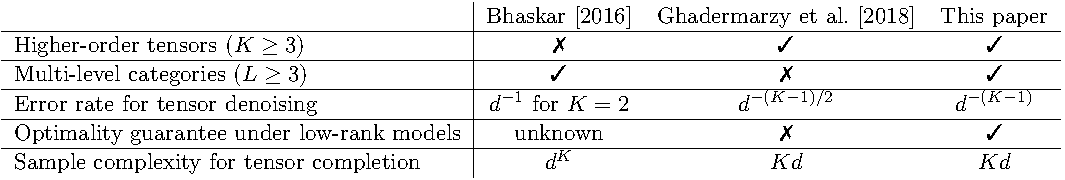
\includegraphics[width=16cm]{compare.pdf}}
\vspace{-.3cm}
\caption{Comparison with previous work. For ease of presentation, we summarize the error rate and sample complexity assuming equal tensor dimension in all modes. $K$: tensor order; $L$: number of ordinal levels; $d$: dimension at each mode. }~\label{tab:compare}
\vspace{-.5cm}
\end{table*}

{\bf Our contribution.} This paper presents an efficient low-rank estimation method and theory for tensors with ordinal-valued entries. Our main contributions are summarized in Table~\ref{tab:compare}. We propose a cumulative link model for higher-order tensors, develop a rank-constrained M-estimator, and obtain theoretical accuracy guarantees. The mean squared error bound is established, and we show that the obtained bound has minimax optimal rate in high dimensions under the low-rank model. Our estimator enjoys a faster convergence rate $\tO(d^{-(K-1)/2})$ than $\tO(d^{-K})$ in~\citet{ghadermarzy2018learning}, which is a substantial improvement as the order $K$ increases. Furthermore, our proposal serves as an efficient completion algorithm that guarantees consistent recovery of an order-$K$ $(d,\ldots,d)$-dimensional low-rank tensor using only $\tilde \tO(Kd)$ noisy, quantized observations.

{\bf Related work.} Our work is related to, but clearly distinctive from, several lines of existing literature. Matrix completion from quantized samples was firstly introduced for binary observations~\cite{cai2013max,davenport2014,bhaskar20151} and then extended to ordinal observations~\cite{bhaskar2016probabilistic}. As we show in Section~\ref{sec:theory}, applying existing matrix methods to an ordinal tensor results in a suboptimal estimator with a slower convergence rate. Therefore, a full exploitation of the tensor structure is necessary; this is the focus of the current paper.

Our work is also connected to non-Gaussian tensor decomposition. Existing work focuses exclusively on univariate observations such as binary- or continuous-valued entries~\citep{wang2018learning,hong2018generalized,ghadermarzy2018learning}. As we mentioned earlier, the ordinal observations add considerable challenges to the model formulation. We address the problems from two perspectives. From statistical perspective, our proposed model generalizes the usual binary tensor model while preserving palindromic invariance~\cite{mccullagh1980regression} for ordinal observations. From algorithm perspective, our alternating optimization compares favorably to the approximate (non-convex) algorithm developed in the context of binary tensors~\cite{ghadermarzy2018learning}. We numerically compare the two approaches in Section~\ref{sec:experiment}.


\section{Preliminaries}
Let $\tY\in\mathbb{R}^{d_1\times \cdots \times d_K}$ denote an order-$K$ $(d_1,\ldots,d_K)$-dimensional tensor. We use $y_\omega$ to denote the tensor entry indexed by $\omega$, where $\omega\in[d_1]\times\cdots\times[d_K]$.  The Frobenius norm of $\tY$ is defined as $\FnormSize{}{\tY}=\sum_\omega y^2_\omega$ and the infinity norm of $\tY$ is defined as $\mnormSize{}{\tY}=\max_{\omega}|y_\omega|$. We use $\tY_{(k)}$ to denote the unfolded matrix of size $d_k$-by-$\prod_{i\neq k}d_k$, obtained by reshaping the tensor along the mode-$k$. The Tucker rank of $\tY$ is defined as a length-$K$ vector $\mr = (r_1,\ldots,r_K)$, where $r_k$ is the rank of matrix $\tY_{(k)}$ for all $k \in[K]$. We say that an event $A$ occurs ``with very high probability'' if $\mathbb{P}(A)$ tends to 1 faster than any polynomial of tensor dimension $d_{\min}=\min\{d_1,\ldots,d_K\} \to\infty$.

We use lower-case letters ($a, b, c, \ldots$) for scalars/vectors, upper-case boldface letters ($\mA, \mB, \mC, \ldots$) for matrices, and calligraphy letters ($\tA,\tB,\tC,\ldots$) for tensors of order three or greater. For ease of notation, we allow the basic arithmetic operators (e.g., $\leq, +, -$) to be applied to pairs of tensors in an element-wise manner. We use the shorthand $[n]$ to denote the $n$-set $\{1,\ldots,n\}$ for $n \in N_{+}$.

\vspace{-.2cm}
\section{Model formulation and motivation}
\subsection{Observation model}
Let $\tY$ denote an order-$K$ $(d_1,\ldots,d_K)$-dimensional data tensor. Suppose the entries of $\tY$ are ordinal-valued, and the observation space consists of $L$ ordered levels, denoted by $[L]:=\{1,\ldots,L\}$. We propose a cumulative link model for the ordinal tensor $\tY=\entry{y_\omega}\in[L]^{d_1\times \cdots\times d_K}$. Specifically, assume the entries $y_\omega$ are (conditionally) independently distributed with cumulative probabilities:
\begin{equation}\label{eq:model}
\mathbb{P}(y_\omega\leq \ell)=f(b_\ell-\theta_\omega),\ \text{for all}\ \ell\in[L-1],
\end{equation}
where $\mb=(b_1,\ldots,b_{L-1})$ is a set of unknown scalars satisfying $b_1<\cdots <b_{L-1}$, $\Theta=\entry{\theta_\omega}\in\mathbb{R}^{d_1\times \cdots \times d_K}$ is a continuous-valued parameter tensor satisfying certain low-dimensional structure (to be specified later), and $f(\cdot):\mathbb{R}\mapsto[0,1]$ is a known, strictly increasing function. We refer to $\mb$ as the cut-off points and $f$ the link function.

The formulation~\eqref{eq:model} imposes an additive model to the transformed probability of cumulative categories. This modeling choice is to respect the ordering structure among the categories. For example, if we choose the inverse link $f^{-1}(x)=\log {x\over 1-x}$ to be the log odds, then the model~\eqref{eq:model} implies linear spacing between the proportional odds:
\begin{equation}\label{eq:logodd}
\log {\mathbb{P}(y_{\omega}\leq \ell) \over \mathbb{P}(y_\omega >  \ell) } - \log {\mathbb{P}(y_{\omega}\leq {\ell-1}) \over \mathbb{P}(y_\omega >  {\ell-1}) } = b_\ell-b_{\ell-1},
\end{equation}
for all tensor entries $y_\omega$. When there are only two categories in the observation space (e.g. binary tensors), the cumulative model~\eqref{eq:model} is equivalent to the usual multinomial link model. In general, however, when the number of categories $L\geq 3$, the proportional odds assumption~\eqref{eq:logodd} is more parsimonious, in that, the ordered categories can be envisaged as contiguous intervals on the continuous scale, where the points of division are exactly $b_1<\cdots <b_{L-1}$. This interpretation will be made more explicit in the next section.

\subsection{Latent-variable interpretation}\label{sec:latent}
The ordinal tensor model~\eqref{eq:model} with certain types of link $f$ has the equivalent representation as an $L$-level quantization model on $\tY=\entry{y_\omega}$:
\begin{align}\label{eq:quantization}
y_\omega&=
\begin{cases}
1,& \text{if $y^*_\omega\in(-\infty, b_1]$},\\
2,& \text{if $y^*_\omega\in(b_1, b_2]$},\\
\vdots  &\vdots\\
L,& \text{if $y^*_\omega\in(b_{L-1}, \infty)$},\\
\end{cases}
\end{align}
for all $\omega\in[d_1]\times \cdots \times [d_k]$. Here, $\tY^*=\entry{y^*_\omega}$ is a latent continuous-valued tensor following an additive noise model:
\begin{align}\label{eq:latent}
\KeepStyleUnderBrace{\tY^*}_{\text{latent continuous-valued tensor}}=\KeepStyleUnderBrace{\Theta}_{\text{signal tensor}}+\KeepStyleUnderBrace{\tE}_{\text{i.i.d.\ noise}},
\end{align}
where $\tE=\entry{\varepsilon_\omega}\in\mathbb{R}^{d_1\times \cdots \times d_K}$ is a noise tensor with i.i.d.\ entries according to distribution $\mathbb{P}(\varepsilon)$. From the viewpoint of~\eqref{eq:latent}, the parameter tensor $\Theta$ can be interpreted as the latent signal tensor prior to contamination and quantization.

The equivalence between the latent-variable model~\eqref{eq:quantization} and the cumulative link model~\eqref{eq:model} is established if the link $f$ is chosen to be the cumulative distribution function of noise $\varepsilon$, i.e., $f(\theta)=\mathbb{P}(\varepsilon\leq \theta)$. We describe two common choices of link $f$, or equivalently, the distribution of $\varepsilon$.

\begin{example}[Logistic model] The logistic model is characterized by~\eqref{eq:model} with $f(\theta)=(1+e^{-\theta/\sigma})^{-1}$, where $\sigma>0$ is the scale parameter. Equivalently, the noise $\varepsilon_\omega$ in~\eqref{eq:quantization} follows i.i.d.\ logistic distribution with scale parameter $\sigma$.
\end{example}
\begin{example}[Probit model] The probit model is characterized by~\eqref{eq:model} with
$f(\theta)=\mathbb{P}(z\leq \theta/\sigma)$, where $z\sim N(0,1)$. Equivalently, the noise $\varepsilon_\omega$ in~\eqref{eq:quantization} follows i.i.d.\ $N(0,\sigma^2)$.
\end{example}
Other link functions are also possible, such as Laplace, Cauchy, etc~\cite{mccullagh1980regression}. All the models share the property that the ordered categories can be thought of as contiguous interval on some continuous scale. We should point out that, although the latent-variable interpretation is incisive, our estimation procedure does not refer to the existence of $\tY^*$. Therefore, our model~\eqref{eq:model} is general and still valid in the absence of quantization process. More generally, we make the following assumptions about the link $f$.

\begin{assumption}\label{ass:link}
The link function is assumed to satisfy:
\vspace{-.4cm}
\begin{enumerate}
\item $f(\theta)$ is strictly increasing and twice-differentiable in $\theta\in\mathbb{R}/\{0\}$.
\vspace{-.2cm}
\item $f'(\theta)$ is strictly log-concave and symmetric with respect to $\theta=0$.
\end{enumerate}
\end{assumption}

\subsection{Problem 1: Tensor denoising}~\label{sec:denoising}
The first question we aim to address is tensor denoising:

(P1) Given the quantization process induced by $f$ and the cut-off points $\mb$, how accurately can we estimate the latent signal tensor $\Theta$ from the ordinal observation $\tY$?

Clearly, the problem (P1) cannot be solved uniformly for all possible $\Theta$. We focus on a class of ``low-rank'' and ``flat'' signal tensors, which is a plausible assumption in practical applications~\cite{zhou2013tensor,bhaskar20151}. Specifically, we consider the parameter space:
\begin{equation}\label{eq:space}
\small \tP=\left\{\Theta\in\mathbb{R}^{d_1\times \cdots \times d_K} \colon \text{rank}(\Theta)\leq \mr,\ \mnormSize{}{\Theta}\leq \alpha\right\}.
\end{equation}
where $\mr=(r_1,\ldots,r_K)$ denotes the Tucker rank of $\Theta$.

The parameter tensor of our interest satisfies two constraints. The first is that $\Theta$ is a low-rank tensor, with $r_k=\tO(1)$ for all $k\in[K]$. Equivalently, $\Theta$ admits the Tucker decomposition:
\begin{equation}\label{eq:Tucker}
\Theta=\tC\times_1\mM_1\times_1 \cdots \times_K \mM_K,
\end{equation}
where $\tC\in\mathbb{R}^{r_1\times \cdots \times r_K}$ is a core tensor, $\mM_k\in\mathbb{R}^{d_k\times r_k}$ are factor matrices with orthogonal columns, and $\times_k$ denotes the tensor-by-matrix multiplication~\cite{kolda2009tensor}. The Tucker low-rankness is popularly imposed in tensor data analysis, and is shown to provide a reasonable tradeoff between model complexity and model flexibility. Note that, unlike matrices, there are various notations of tensor low-rankness, such as CP rank~\cite{hitchcock1927expression} and train rank~\cite{oseledets2011tensor}. Some notation of low-rankness may lead to mathematically ill-posed optimization; for example, the best low CP-rank tensor approximation may not exist~\cite{de2008tensor}. We choose Tucker representation for well-posedness of optimization and easy interpretation.

The second constraint is that the entries of $\Theta$ are uniformly bounded in magnitude by a constant $\alpha \in \mathbb{R}_{+}$. In view of~\eqref{eq:latent}, we refer to $\alpha$ as the signal level. The entry-wise bound assumption is a technical condition that avoids the degeneracy in probability estimation with ordinal observations.

\subsection{Problem 2: Tensor completion}
Motivated by applications in collaborative filtering, we also consider a more general setup when only a subset of tensor entries $y_\omega$ are observed. Let $\Omega\subset[d_1]\times \cdots\times[d_K]$ denote the set of observed indices. The second question we aim to address is stated as follows:

(P2) Given an incomplete set of ordinal observations $\{y_{\omega}\}_{\omega\in\Omega}$, how many sampled entries do we need to consistently recover $\Theta$ based on the model~\eqref{eq:model}?

The answer to (P2) depends on the choice of $\Omega$. We consider a general model on $\Omega$ that allows both uniform and non-uniform sampling. Specifically, let $\Pi=\{\pi_{i_1,\ldots,i_K}\}$ denote a predefine probability distribution over the index set such that $\sum_{\omega\in[d_1]\times \cdots \times [d_K]} \pi_\omega =1$. We assume that each index in $\Omega$ is drawn with replacement using distribution $\Pi$. This sampling model relaxes the uniform sampling in literature and is arguably a better fit in applications.

We consider the same parameter space~\eqref{eq:space} for the completion problem. In addition to the reasons mentioned in Section~\ref{sec:denoising}, the entrywise bound assumption also serves as the incoherence requirement for completion. In classical matrix completion, the incoherence is often imposed on the singular vectors. This assumption is recently relaxed for ``flat'' matrices with bounded magnitude~\cite{negahban2011estimation,cai2013max,bhaskar20151}. We adopt the same assumption for higher-order tensors.

\section{Rank-constrained M-estimator}\label{sec:theory}
We present a general treatment to both problems mentioned above. With a little abuse of notation, we use $\Omega$ to denote either the full index set $\Omega=[d_1]\times \cdots \times [d_K]$ (for the tensor denoising) or a random subset induced from the sampling distribution $\Pi$ (for the tensor completion). Define $b_0=-\infty$, $b_L=\infty$, $f(-\infty)=0$ and $f(\infty)=1$. The log-likelihood associated with the observed entries is
\begin{align}\label{eq:objective}
\logl(\Theta, \mb)&=\sum_{\omega\in\Omega}\sum_{\ell\in[L]} \Big\{\mathds{1}_{\{y_\omega=\ell\}} \log \big[f(b_\ell-\theta_\omega)- \notag \\
&\quad \quad \quad \quad \quad \quad \quad  f(b_{\ell-1}-\theta_\omega)\big]\Big\}.
\end{align}
We propose a rank-constrained maximum likelihood estimator (a.k.a.\ M-estimator) for $\Theta$:
\begin{align}\label{eq:estimator}
\hat \Theta&=\argmax_{\Theta\in \tP}\logl(\Theta, \mb),\ \text{where}\notag \\
\tP&=\left\{\Theta\in\mathbb{R}^{d_1\times \cdots \times d_K} \colon \text{rank}(\Theta)\leq \mr,\ \mnormSize{}{\Theta}\leq \alpha\right\}.
 \end{align}
In practice, the cut-off points $\mb$ are unknown and should be jointly estimated with $\Theta$. For technical convenience, we assume in this section that the cut-off points $\mb$ are known. The adaptation of unknown $\mb$ is addressed in Section~\ref{sec:algorithm} and the Supplement.

We define a few key quantities that will be used in our theory. Let $g_\ell=f(\theta+b_\ell)-f(\theta+b_{\ell-1})$ for all $\ell\in[L]$, and
\begin{align}\label{eq:regular}
A_\alpha &= \min_{\ell\in[L], |\theta|\leq \alpha} g_\ell(\theta),\quad  U_\alpha=\max_{\ell\in[L], |\theta|\leq \alpha } {\dot{g}_\ell(\theta)\over g_\ell(\theta)},\\
 L_\alpha &= \min_{\ell\in[L], |\theta|\leq \alpha }\left[{\dot{g}_\ell^2 (\theta)\over g_\ell^2(\theta)} -{\ddot{g}_\ell(\theta)\over g_\ell(\theta)}\right],
\end{align}
where $\dot{g}(\theta)=dg(\theta)/d\theta$, and $\alpha$ is the entrywise bound of $\Theta$. In view of equation~\eqref{eq:latent}, these quantities characterize the geometry including flatness and convexity of the latent noise distribution. Under the Assumption~\ref{ass:link}, all these quantities are strictly positive and independent of tensor dimension.

\subsection{Estimation error for tensor denoising}\label{sec:denosing}
For the tensor denoising problem, we assume that the full set of tensor entries are observed. We assess the estimation accuracy using the mean squared error (MSE):
\[
\text{MSE}(\hat \Theta, \trueT)={1\over \prod_k d_k}\FnormSize{}{\Theta-\trueT}^2.
\]
The next theorem establishes the upper bound for the MSE of the proposed $\hat \Theta$ in~\eqref{eq:estimator}.

\begin{thm}[Statistical convergence] \label{thm:rate}
Consider an ordinal tensor $\tY\in[L]^{d_1\times\dots\times d_K}$ generated from model~\eqref{eq:model}, with the link function $f$ and the true coefficient tensor $\trueT\in\tP$. Define $r_{\max}=\max_k r_k$. Then, with very high probability, the estimator in~\eqref{eq:estimator} satisfies
\begin{equation}\label{eq:rate}
\text{MSE}(\hat \Theta, \trueT) \leq \min\left( 4\alpha^2,\ {c_2  U^2_\alpha r_{\max}^{K-1}  \over  L^2_\alpha } {\sum_kd_k\over  \prod_k d_k} \right),
\end{equation}
where $c_1, c_2>0$ are two constants that depend only on $K$.
\end{thm}
Theorem~\ref{thm:rate} establishes the statistical convergence for the estimator~\eqref{eq:estimator}. In fact, the proof of this theorem (see the Supplement) shows that the same statistical rate holds, not only for the global optimizer~\eqref{eq:estimator}, but also for any local optimizer $\check \Theta$ in the level set $\{\check\Theta\in\tP: \logl(\check\Theta)\geq \logl(\trueT)\}$. This suggests that the local optimality itself is not necessarily a severe concern in our context, as long as the convergent objective is large enough. In Section ~\ref{sec:algorithm}, we perform empirical studies to assess the algorithmic stability.

A similar conclusion is obtained for the prediction error, measured in Kullback-Leibler (KL) divergence, between the categorical distributions in the observation space.
\begin{cor}[Prediction error]~\label{cor:prediction}
Assume the same set-up as in Theorem~\ref{thm:rate}. Let $\mathbb{P}_{\tY}$ and $\hat{\mathbb{P}}_{\tY}$ denote the distributions generating the $L$-level ordinal tensor $\tY$, given the true parameter $\Theta$ and its estimator $\hat \Theta$, respectively. Assume $L\geq 2$. Then, with very high probability,
\begin{equation}\label{eq:KLrate}
\text{KL}(\mathbb{P}_{\tY} || \hat{\mathbb{P}}_{\tY}) \leq  {c_2 U^2_\alpha r_{\max}^{K-1}  \over L^2_\alpha } {(4L-6)\dot{f}^2(0)  \over A_\alpha} {\sum_kd_k\over  \prod_k d_k},
\end{equation}
where $c_1, c_2>0$ are the same constants as in Theorem~\ref{thm:rate}.
\end{cor}
To gain insight into these bounds, we consider a special setting with equal dimension in all modes, i.e., $d_1=\cdots=d_K=d$. In such a case, our bound \eqref{eq:rate} reduces to
\begin{equation*}\label{eq:ours}
\text{MSE}(\hat \Theta, \trueT) \asymp d^{-(K-1)}, \quad \text{as}\ d\to \infty.
\end{equation*}
Hence, our estimator achieves consistency with polynomial convergence rate. We compare the bound with existing literature. In the special case $L=2$, \citet{ghadermarzy2018learning} proposed a max-norm constrained estimator $\tilde{\Theta}$ with $\text{MSE}(\tilde{\Theta}, \trueT) \asymp  d^{-(K-1)/2}$. In contrast, our estimator converges at a rate of $d^{-(K-1)}$, which is substantially faster than theirs. This provides a positive answer to the open question posed in~\citet{ghadermarzy2018learning} whether the square root in the bound is removable. The improvement stems from utilizing the exact low-rankness of $\Theta$, whereas the surrogate rank measure employed in~\citet{ghadermarzy2018learning} is scale-sensitive.

Our bound also generalizes the previous results on ordinal matrices. The convergence rate for rank-constrained matrix estimation was $\tO(1/\sqrt{d})$~\citep{bhaskar2016probabilistic}, which fits into our special case when $K=2$. Furthermore, our results~\eqref{eq:rate} and~\eqref{eq:KLrate} reveal that the convergence becomes favorable as the order of data tensor increases. Intuitively, the sample size for tensor data analysis is the number of entries, $\prod_k d_k$, and the number of free parameters is roughly on the order of $\sum_{k}d_k$, assuming $r_{\max}=\tO(1)$. A higher tensor order implies higher effective sample size per parameter, and thus exhibits a faster convergence rate in high dimensions.


We next show the statistical optimality of our estimator $\hat \Theta$. The result is based on the information theory, and applies to all estimators in $\tP$, including but not limited to $\hat \Theta$ in~\eqref{eq:estimator}.


\begin{thm}[Minimax lower bound]\label{thm:minimax}
Assume the same set-up as in Theorem~\ref{thm:rate}, and $d_{\max}=\max_k d_k \geq 8$. Let $\inf_{\hat \Theta}$ denote the infimum over all estimators $\hat \Theta\in\tP$ based on the ordinal tensor observation $\tY\in[L]^{d_1\times \cdots \times d_K}$. Then, under the model~\eqref{eq:model},
\begin{align}\label{eq:lower}
\inf_{\hat \Theta }\sup_{\trueT\in\tP} \mathbb{P}\Big\{& \text{MSE}(\hat \Theta, \trueT) \\
& \geq {1\over 256} \min\left( \alpha^2, \ { Cr_{\max}d_{\max} \over \prod_k d_k} \right) \Big\} \geq {1\over 8},
\end{align}
where $C=C(\alpha, L, f,\mb)>0$ is a constant independent of tensor dimension and the rank.
\end{thm}
We see that the lower bound matches the upper bound in~\eqref{eq:rate} on the polynomial order of tensor dimension. Therefore, our estimator~\eqref{eq:estimator} is order-optimal.

\subsection{Sample complexity for tensor completion}
We now consider the tensor completion problem, when only a subset of entries $\Omega$ are observed. We consider a general sampling procedure induced by $\Pi$. The recovery accuracy is assessed by the weighted squared error:
\begin{align}\label{eq:weighted}
\PiFnormSize{}{\Theta-\hat \Theta}^2&\stackrel{\text{def}}{=}
{1\over |\Omega|}\mathbb{E}_{\Omega\sim \Pi}\FnormSize{}{\Theta-\hat \Theta}^2\notag \\
&=\sum_{\omega\in[d_1]\times \cdots \times [d_K]} \pi_{\omega}(\Theta_{\omega}-\hat \Theta_{\omega})^2.
\end{align}

Note that the recovery error depends on the distribution $\Pi$. In particular, tensor entries with higher sampling probabilities have more influence on the recovery accuracy, compared to the ones with lower sampling probabilities.

\begin{rmk} If we assume each entry is sampled with strictly positive probability; i.e.\ there exits a constant $\mu> 0$ s.t.
\[
\ \pi_\omega\geq {1\over \mu \prod_k d_k},\quad \text{for all}\ \omega\in[d_1]\times\cdots \times [d_K],
\]
then the error in~\eqref{eq:weighted} provides an upper bound for MSE:
\[
\PiFnormSize{}{\Theta-\hat \Theta}^2 \geq {\FnormSize{}{\Theta-\hat \Theta}^2\over \mu \prod_kd_k}={1\over \mu}\text{MSE}(\hat \Theta, \trueT).
\]
The equality is attained under uniform sampling with $\mu=1$.
\end{rmk}


\begin{thm}~\label{thm:completion}
Assume the same set-up as in Theorem~\ref{thm:rate}. Suppose that we observe a subset of tensor entries $\{y_\omega\}_{\omega\in\Omega}$, where $\Omega$ is chosen at random with replacement according to a probability distribution $\Pi$. Let $\hat \Theta$ be the solution to~\eqref{eq:estimator}, and assume $r_{\max}=\tO(1)$. Then, with very high probability,
\[
\PiFnormSize{}{\Theta-\hat \Theta}^2 \to 0,\quad \text{ as }\quad {|\Omega|\over \sum_k d_k} \ \to \infty.
\]
\end{thm}
Theorem~\ref{thm:completion} shows that our estimator achieves consistent recovery using as few as $\tilde{\tO}(Kd)$ noisy, quantized observations from an order-$K$ $(d,\ldots,d)$-dimensional tensor. Note that $\tilde \tO(Kd)$ roughly matches the degree of freedom for an order-$K$ tensor of fixed rank $\mr$, suggesting the optimality of our sample requirement. This sample complexity substantially improves over earlier result $\tO(d^{\lceil K/2\rceil})$ based on square matricization~\cite{mu2014square}, or $\tO(d^{N/2})$ based on tensor nuclear-norm regularization~\cite{yuan2016tensor}. Existing methods that achieve $\tilde \tO(Kd)$ sample complexity require either a deterministic cross sampling design~\cite{zhang2019cross} or univariate measurements~\cite{ghadermarzy2018learning}. Our method extends the conclusions to multi-level measurements under a broader class of sampling schemes.

\vspace{-.2cm}
\section{Numerical Implementation}\label{sec:algorithm}
We describe the algorithm to seek the optimizer of~\eqref{eq:objective}. In practice, the cut-off points $\mb$ are often unknown, so we choose to maximize $\logl$ jointly over $(\Theta,\mb)\in\tP\times \tB$. The objective $\logl$ is concave in $(\Theta,\mb)$ whenever $f'$ is log-concave (see the Supplement). However, the feasible set $\tP$ is non-convex, which makes the optimization~\eqref{eq:objective} a non-convex problem. We employ the alternating optimization approach by utilizing the Tucker representation of $\Theta$. Specifically, based on~\eqref{eq:Tucker} and~\eqref{eq:objective}, the objective function consists of $K+2$ blocks of variables, one for the cut-off points $\mb$, one for the core tensor $\tC$, and $K$ for the factor matrices $\mM_k$'s. The optimization is a simple convex problem if any $K+1$ out of the $K+2$ blocks are fixed. We update one block at a time while holding others fixed, and alternate the optimization throughout the iteration. The convergence is guaranteed whenever $\logl$ is bounded from above, since the alternating procedure monotonically increases the objective. The Algorithm~\ref{alg} gives the full description.

\begin{algorithm}[t]
        \caption{Ordinal tensor decomposition}\label{alg}
        \begin{algorithmic}[]
            \STATE{\bfseries Input:}  \text{ Ordinal data tensor }
            $\mathcal{Y}\in [L]^{d_1\times\cdots\times d_K}$, rank $\mr\in \mathbb{N}_{+}^{K}$, entry-wise bound $\alpha\in \mathbb{R_+}$.
            \STATE{\bfseries Output:} $(\hat\Theta,\hat{\mb}) =  \argmax_{(\Theta,\mb)\in \mathcal{P}\times\mathcal{B}}  \mathcal{L}_{\mathcal{Y},\Omega}(\Theta,\mb).$
            \STATE Random initialization of core tensor $\mathcal{C}^{(0)}$, factor matrices $ \{\mM_k^{(0)}\}$, and cut-off points $\mb^{(0)}$.
            \FOR{$t = 1,2,\cdots,$}
            \FOR{$k = 1,2,\cdots,K$}
            \STATE{Update $\mM^{(t+1)}_k$ while fixing other blocks:}
            \STATE $\mM_k^{(t+1)}\gets\argmax_{\mM_k\in\mathbb{R}^{d_k\times r_K}}\mathcal{L}_{\mathcal{Y},\Omega}(\mM_k)$,
            \newline
             s.t. $\mnormSize{}{\Theta^{(t+1)}}\leq \alpha$, where $\Theta^{(t+1)}$ is the parameter tensor based on the current block estimates.
            \ENDFOR
            \STATE {Update $\mathcal{C}^{(t+1)}$ while fixing other blocks:}
              \newline$\mathcal{C}^{(t+1)} \gets \argmax_{\mathcal{C}\in \mathbb{R}^{r_1\times\cdots\times r_K}}\mathcal{L}_{\mathcal{Y},\Omega}(\mathcal{C})$, s.t. $\mnormSize{}{\Theta^{(t+1)}}\leq \alpha.$
               \STATE {Update $\Theta^{(t+1)}$ based on the current block estimates:}
                   \newline
                   $\Theta^{(t+1)} \gets \mathcal{C}^{(t+1)}\times_1\mM_1^{(t+1)}\cdots\times_K\mM_K^{(t+1)}.$
            \STATE {Update $\mb^{(t+1)}$ while fixing $\Theta^{(t+1)}$:}
              \newline
              $\mb^{(t+1)} \gets \argmax_{\mb\in \tB}\mathcal{L}_{\mathcal{Y},\Omega}\big(\Theta^{(t+1)},\mb\big).$
            \ENDFOR
            \STATE \textbf{return}
            $(\hat \Theta,\hat \mb)$
        \end{algorithmic}
 \end{algorithm}
We comment on two implementation details before concluding this section. First, the problem~\eqref{eq:estimator} is non-convex, so Algorithm 1 usually has no theoretical guarantee on global optimality. Nevertheless, as shown in Section~\ref{sec:denosing}, the desired rate holds not only for the global optimizer, but also for the local optimizer with $\logl(\hat \Theta)\geq \logl(\trueT)$. In practice, we find the convergence point $\hat \Theta$ upon random initialization is often satisfactory, in that the corresponding objective $\logl(\hat \Theta)$ is close to and actually slightly larger than the objective evaluated at the true parameter $\logl(\trueT)$. Figure~\ref{fig:stability} shows the trajectory of the objective function that is output in the default setting of Algorithm 1, with the input tensor generated from probit model~\eqref{eq:model} with $d_1=d_2=d_3=d$ and $r_1=r_2=r_3=r$. The dashed line is the objective value at the true parameter $\logl(\trueT)$. We find that the algorithm generally converges quickly to a desirable value in reasonable number of steps. The actual running time per iteration is shown in the plot legend.

\begin{figure}[H]
\centering
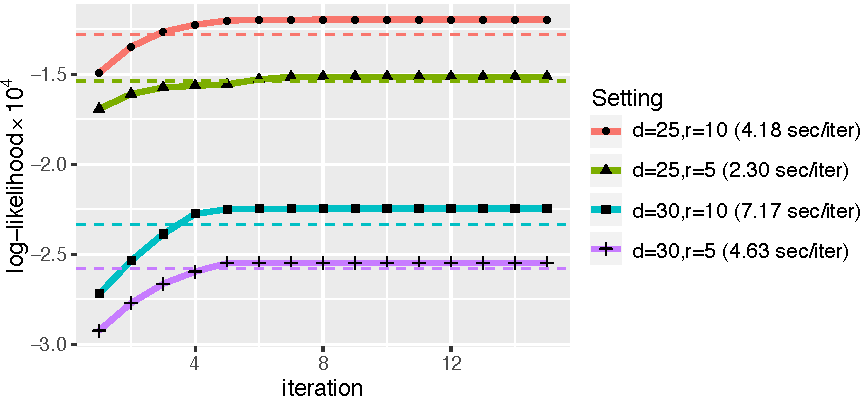
\includegraphics[width=8cm]{algorithm.pdf}\label{fig:stability}
\vspace{-.2cm}
\caption{Trajectory of objective function with various $d$ and $r$.}
\vspace{-.5cm}
\end{figure}



Second, the algorithm takes the rank $\mr$ as an input. In practice, the rank $\mr$ is hardly known and needs to be estimated from the data. We suggest to use Bayesian information criterion (BIC) and choose the rank that minimizes BIC; i.e.
\begin{align}\label{eq:BIC}
\hat \mr&=\argmin_{\mr\in\mathbb{N}^K_{+}} \text{BIC}(\mr)\\
&=\argmin_{\mr\in\mathbb{N}^K_{+}}\{-2\tL_{\tY}(\hat \Theta(\mr),\hat \mb(\mr))+p_e(\mr)\log (\prod_k d_k)\},
\end{align}
where $\hat \Theta(\mr), \hat\mb(\mr)$ are the estimates given the rank $\mr$, and $p_e(\mr)\stackrel{\text{def}}{=}\sum_k (d_k-r_k)r_k+\prod_k r_k$ is the effective number of parameters in the model. We select $\hat \mr$ that minimizes BIC through a grid search. The choice of BIC is intended to balance between the goodness-of-fit for the data and the degrees of freedom in the population model.

\vspace{-.2cm}
\section{Experiments}\label{sec:experiment}
In this section, we evaluate the empirical performance of our method. We investigate both the complete and the incomplete settings, and compare the recovery accuracy with other tensor-based methods. Unless otherwise stated, the ordinal data tensors are generated from model~\eqref{eq:model} using standard probit link $f$. We consider the setting with $K=3$, $d_1=d_2=d_3=d$, and $r_1=r_2=r_3=r$. The parameter tensors are simulated based on~\eqref{eq:Tucker}, where the core tensor entries are i.i.d.\ drawn from $N(0,1)$, and the factors $\mM_k$ are uniformly sampled (with respect to Haar measure) from matrices with orthonormal columns. We set the cut-off points $b_\ell=f^{-1}(\ell/L)$ for $\ell\in[L]$, such that $f(b_\ell)$ are evenly spaced from 0 to 1. In each simulation study, we report the summary statistics across $n_{\text{sim}}$ = 30 replications.

\vspace{-.1cm}
\subsection{Finite-sample performance}\label{sec:simulation}
\vspace{-.1cm}
The first experiment examines the performance under complete observations. We assess the empirical relationship between the MSE and various aspects of model complexity, such as dimension $d$, rank $r$, and signal level $\alpha=\mnormSize{}{\Theta}$. Figure~\ref{fig:finite}a plots the estimation error versus the tensor dimension $d$ for three different ranks $r\in\{3,5,8\}$. The decay in the error appears to behave on the order of $d^{-2}$, which is consistent with our theoretical results~\eqref{eq:rate}. We find that a higher rank leads to a larger error, as reflected by the upward shift of the curve as $r$ increases. Indeed, a higher rank implies the higher number of parameters to estimate, thus increasing the difficulty of the estimation. Figure~\ref{fig:finite}b shows the estimation error versus the signal level under $d=20$. Interestingly, a larger estimation error is observed when the signal is either too small or too large. The non-monotonic behavior may seem surprising, but this is an intrinsic feature in the estimation with ordinal data. In view of the latent-variable interpretation (see Section~\ref{sec:latent}), estimation from ordinal observation can be interpreted as an inverse problem of quantization. Therefore, the estimation error diverges in the absence of noise $\tE$, because it is impossible to distinguish two different signal tensors, e.g., $\Theta_1=\ma_1\otimes \ma_2\otimes \ma_3$ and $\Theta_2=\text{sign}(\ma_1)\otimes \text{sign}(\ma_2)\otimes \text{sign}(\ma_3)$, from the quantized observations. This phenomenon~\cite{davenport2014,sur2019modern} is clearly contrary to the classical continuous-valued tensor problem.

The second experiment investigates the incomplete observations. We consider $L$-level tensors with $d=20$, $\alpha=10$ and choose a subset of tensor entries via uniform sampling. Figure~\ref{fig:finite}c shows the estimation error of $\hat \Theta$ versus the fraction of observation $\rho=|\Omega|/d^K$. As expected, the error reduces with increased $\rho$ or decreased $r$. Figure~\ref{fig:finite}d evaluates the impact of ordinal levels $L$ to estimation accuracy, under the setting $\rho=0.5$. An improved performance is observed as $L$ grows, especially from binary observations ($L=2$) to multi-level ordinal observations ($L\geq 3$). The result showcases the benefit of multi-level observations compared to binary observations.

\begin{figure}[http]
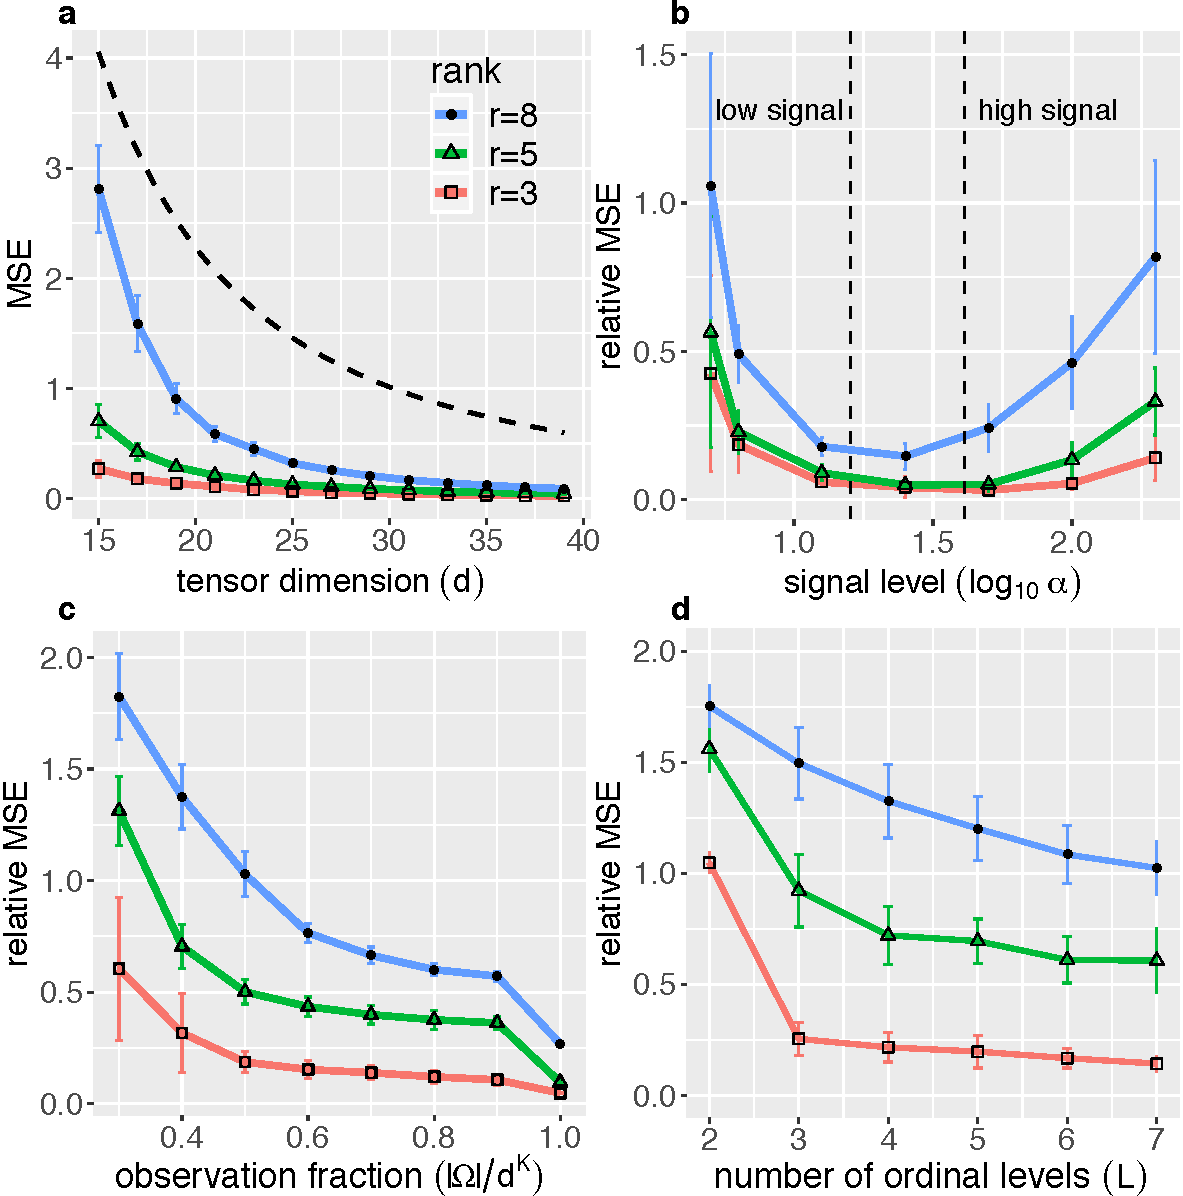
\includegraphics[width=8.3cm]{panel.pdf}
\vspace{-.4cm}
\caption{Empirical relationship between (relative) MSE versus (a) dimension $d$, (b) signal level $\alpha$, (c) observation fraction $\rho$, and (d) number of ordinal levels $L$. In panels (b)-(d), we plot the relative MSE $=\FnormSize{}{\hat \Theta-\trueT}/\FnormSize{}{\trueT}$ for better visualization.}
\label{fig:finite}
\vspace{-.2cm}
\end{figure}

\vspace{-.1cm}
\subsection{Comparison with alternative methods}
\vspace{-.1cm}
Next, we compare our ordinal tensor method ({\bf Ordinal-T}) with three popular low-rank methods:

\begin{itemize}[itemsep=-.5pt,topsep=-.5pt,leftmargin=*,partopsep=-.5pt]
\item Continuous tensor decomposition ({\bf Continuous-T})~\cite{acar2010scalable} is a low-rank approximation method based on classical Tucker model.
\item One-bit tensor completion ({\bf 1bit-T})~\cite{ghadermarzy2018learning} is a max-norm penalized tensor learning method based on partial binary observations.
\item Ordinal matrix completion ({\bf Ordinal-M})~\cite{bhaskar2016probabilistic} is a rank-constrained matrix estimation method based on noisy, quantized observations.
\end{itemize}

We apply each of the above methods to $L$-level ordinal tensors $\tY$ generated from model~\eqref{eq:model}. The {\bf Continuous-T} is applied directly to $\tY$ by treating the $L$ levels as continuous observations. The {\bf Ordinal-M} is applied to the matrix $\tY_{(1)}$ obtained via 1-mode unfolding. The {\bf 1bit-T} is applied to $\tY$ in two ways. The first approach ({\bf 1bit-sign-T}) follows from~\citet{ghadermarzy2018learning} that transforms
$\tY$ to a binary tensor, by taking the entrywise sign of the mean-adjusted tensor, $\tY- |\Omega|^{-1}\sum_\omega y_\omega$. The second approach ({\bf 1bit-category-T}) transforms the order-3 ordinal tensor $\tY$ to an order-4 binary tensor $\tY^{\sharp}=\entry{y^{\sharp}_{ijkl}}$ via dummy variable encoding; i.e., $y^{\sharp}_{ijk\ell}=\mathds{1}_{\{y_{ijk}=\ell\}}$ for all $\ell\in[L-1]$.
We evaluate the methods by their capabilities in predicting the most likely label for each entry, i.e.,\ $y_\omega^{\text{mode}}=\arg\max_\ell\mathbb{P}(y_\omega=\ell)$. Two performance metrics are considered: mean absolute deviation, $\text{MAD}=d^{-K}\sum_\omega |y_\omega^{\text{mode}}-\hat y_\omega^{\text{mode}}|$, and misclassification rate, $\text{MCR}=d^{-K}\sum_\omega\mathds{1}_{\{y_\omega^{\text{mode}}\neq\text{round}(\hat y_\omega^{\text{mode}})\}}$,
where $\text{round}(\cdot)$ denotes the nearest integer of the prediction (possibly continuous-valued returned by {\bf Continuous-T}). Note that MAD penalizes the large deviation more heavily than MCR.


Figure~\ref{fig:compare} compares the prediction accuracy under the setting $\alpha=10$, $d=20$, and $r=5$. The problem size we considered is comparable to~\citet{ghadermarzy2018learning}. We find that our method outperforms the others in both MAD and MCR. In particular, methods built on multi-level observations ({\bf Ordinal-T}, {\bf Ordinal-M}, {\bf 1bit-category-T}) exhibit stable MCR over $\rho$ and $L$, whereas the others two methods ({\bf Continuous-T}, {\bf 1bit-sign-T}) generally fail except for $L=2$ (Figures~\ref{fig:compare}a-b). This observation highlights the necessity of modeling multi-level probabilities in classification task. Interestingly, although both {\bf 1bit-category-T} and our method {\bf Ordinal-T} behave similarly for binary tensors ($L=2$), the improvement of our method is substantial as $L$ increases (Figures~\ref{fig:compare}a and~\ref{fig:compare}c). One possible reason is that our method incorporates the intrinsic ordering among the $L$ levels via proportional odds assumption~\eqref{eq:logodd}, whereas {\bf 1bit-category-T} ignores the ordinal structure and dependence among the induced binary entries. Figures~\ref{fig:compare}c-d assess the prediction accuracy with sample size. We see a clear advantage of our method ({\bf Ordinal-T}) over the matricization ({\bf Ordinal-M}) in both complete and non-complete observations. When the observation fraction is small, e.g., ${|\Omega|/ d^K}=0.4$, the tensor-based completion shows $\sim$ 30\% reduction in error compared to the matricization.


\begin{figure}[t]
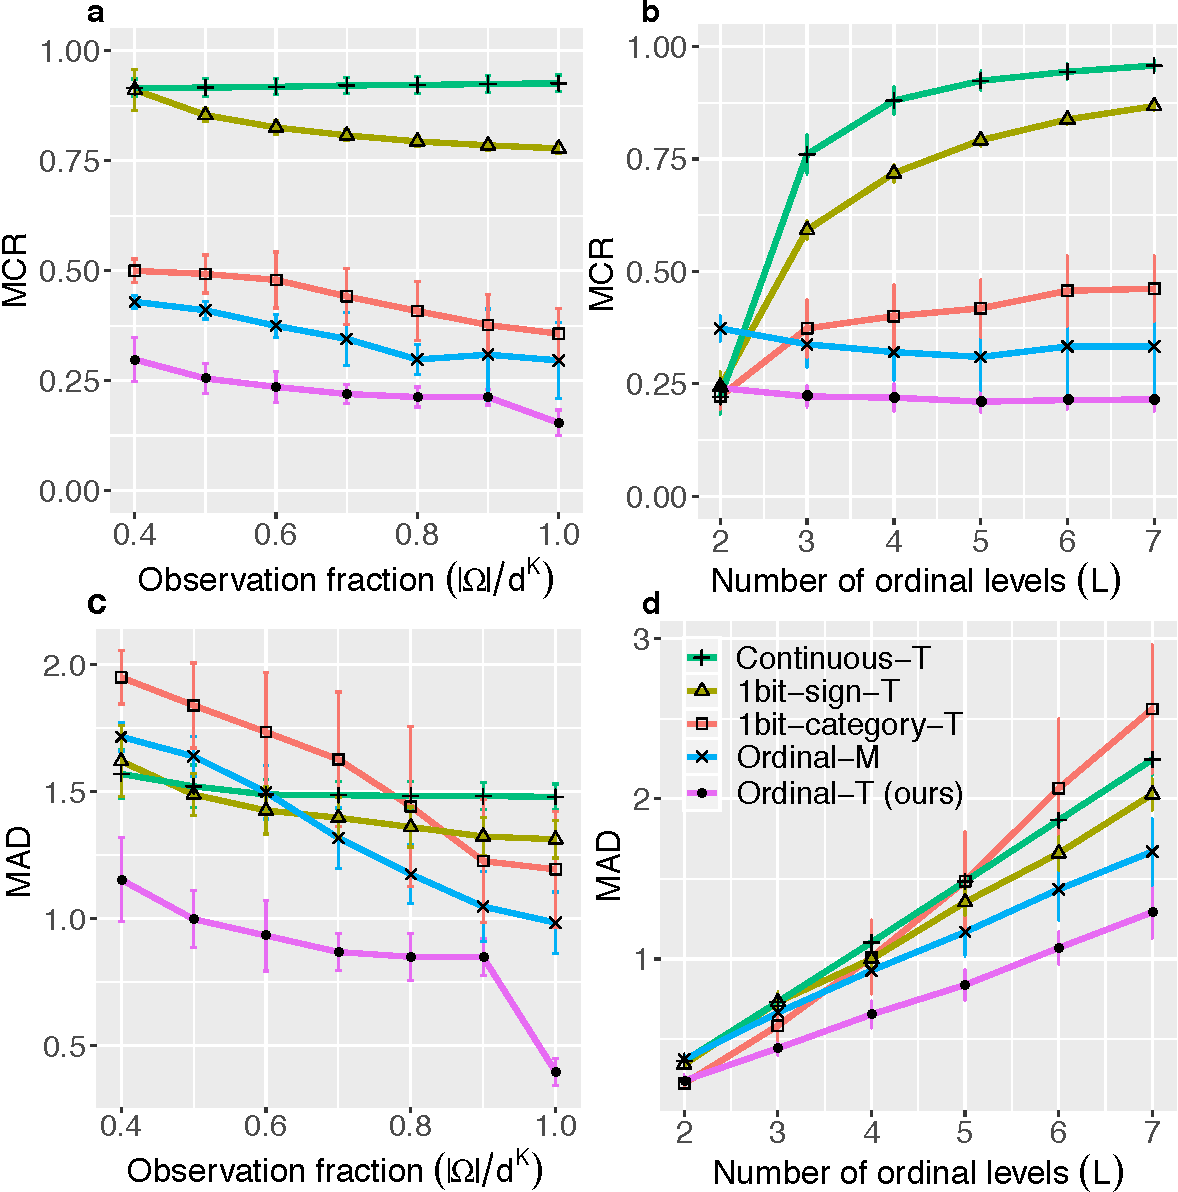
\includegraphics[width=8.3cm]{panel2.pdf}
\vspace{-.4cm}
\caption{Performance comparison in MCR (a, b) and MAD (c, d). (b, d) Prediction errors versus the number of ordinal levels $L$ when $\rho=0.8$. (a, c) Prediction errors versus sample complexity $\rho=|\Omega|/d^K$ when $L=5$. }\label{fig:compare}
\vspace{-.6cm}
\end{figure}


We also compare the methods by their performance in predicting the median label, $y_\omega^{\text{median}}=\min\{\ell\colon\mathbb{P}(y_\omega=\ell)\geq 0.5\}$. Under the latent variable model~\eqref{eq:latent} and Assumption~\ref{ass:link}, the median label is the quantized $\Theta$ without noise; i.e.\ $y_\omega^{\text{median}}=\sum_\ell \mathds{1}_{\theta_\omega\in(b_{\ell-1},b_\ell]}$. Similar results demonstrate the outperformance of our method (see the Supplement).

\vspace{-.1cm}
\section{Data Applications}
\vspace{-.1cm}
We apply our ordinal tensor method to two real-world datasets. In the first application, we use our model to analyze an ordinal tensor consisting of structural connectivities among 68 brain regions for 136 individuals from Human Connectome Project (HCP)~\citep{geddes2016human}. In the second application, we perform tensor completion to an ordinal dataset with missing values. The data tensor records the ratings on a scale of 1 to 5 from 42 users to 139 songs on 26 contexts~\citep{baltrunas2011incarmusic}.

\vspace{-.1cm}
\subsection{Human Connectome Project (HCP)}
\vspace{-.1cm}
Each entry in the HCP dataset takes value on a nominal scale, \{{\it high, moderate, low}\}, indicating the strength level of fiber connection. We convert the dataset to a 3-level ordinal tensor $\tY\in[3]^{68\times 68\times 136}$ and apply the ordinal tensor method with a logistic link function. The BIC suggests $\mr = (23,23,8)$ with $\logl(\hat{\Theta},\hat{\mb}) = -216,646$. Based on the estimated Tucker factors $\{\hat \mM_k\}$, we perform a clustering analysis via K-mean on the brain nodes (see detailed procedure in the Supplement). We find that the 68 brain nodes are grouped into eight clusters, and the clustering capture the spatial separation of brain nodes very well (see the Supplement). In particular, the top two clusters represent the left and right hemispheres; the smaller clusters represent local regions driving by similar nodes. For example, the cluster IV consists of brain nodes {\it postcentral}, {\it posteriorcingulate}, {\it pericalcarine} and {\it temporalpole}, all of which are located at {\it SupraM}. The identified similarity among brain nodes suggests the applicability of our method.

We compare the goodness-of-fit of various tensor methods on the HPC data. Table~\ref{table:CV} summarizes the prediction error via 5-fold stratified cross-validation averaged over 10 runs. Our method outperforms the others, especially in MAD.

\begin{table}[http]
\resizebox{.48\textwidth}{!}{
\begin{tabular}{c|c|c}
\Xhline{2\arrayrulewidth}
\multicolumn{3}{c}{Human Connectome Project (HCP) dataset}\\
\Xhline{2\arrayrulewidth}
Method                    & MAD & MCR\\
\hline
Ordinal-T (ours) & 0.1607 (0.0005)& 0.1606 (0.0005)\\
 Continuous-T&0.2530 (0.0002)&0.1599 (0.0002)\\
 1bit-sign-T&0.3566 (0.0010)&0.1563 (0.0010)\\
 \Xhline{2\arrayrulewidth}
\multicolumn{3}{c}{InCarMusic dataset}\\
\Xhline{2\arrayrulewidth}
Method                    & MAD & MCR\\
\hline
Ordinal-T (ours) & 1.37 (0.039) &  0.59 (0.009)\\
Continuous-T & 2.39 (0.152)&0.94 (0.027)\\
1bit-sign-T&1.39 (0.003)& 0.81 (0.005)\\
\hline
\end{tabular}
}
\vspace{-.2cm}
\caption{Comparison of prediction error in the HPC and InCarMusic analyses. Standard errors are reported in parentheses.}\label{table:CV}
\vspace{-.3cm}
\end{table}

\vspace{-.1cm}
\subsection{InCarMusic recommendation system}
\vspace{-.1cm}
We apply ordinal tensor completion to a recommendation system {\it InCarMusic}. {\it InCarMusic} is a mobile application that offers music recommendation to passengers of cars based on contexts~\cite{baltrunas2011incarmusic}. Our goal is to perform tensor completion to impute the unobserved entries in the $42\times 139\times 26$ ordinal tensor and thereby we can offer context-specific music recommendation to users. The data tensor consists of 2,884 observed entries. Table~\ref{table:CV} shows the averaged prediction error via 5-fold cross validation. The high missing rate makes the accurate classification challenging. Nevertheless, our method achieves the best performance among the three.

\vspace{-.2cm}
\section{Conclusions}
\vspace{-.1cm}
We have developed a low-rank tensor estimation method based on possibly incomplete, ordinal-valued observations. A sharp error bound is established, and we demonstrate the outperformance of our approach compared to other methods. The work unlocks several directions of future research. One interesting question would be the inference problem, i.e.. to assess the uncertainty of the obtained estimates and the imputation. Other directions include the trade-off between (non)convex optimization and statistical/computational efficiency. While convex relaxations are popular approach for matrix-based problem, they are often slow in practice~\cite{chen2019non}. The interplay between computational efficiency and statistical accuracy in general tensor problems warrants future research.

\newpage
\bibliography{tensor_wang}
\bibliographystyle{icml2020}


\end{document}


% This document was modified from the file originally made available by
% Pat Langley and Andrea Danyluk for ICML-2K. This version was created
% by Iain Murray in 2018, and modified by Alexandre Bouchard in
% 2019 and 2020. Previous contributors include Dan Roy, Lise Getoor and Tobias
% Scheffer, which was slightly modified from the 2010 version by
% Thorsten Joachims & Johannes Fuernkranz, slightly modified from the
% 2009 version by Kiri Wagstaff and Sam Roweis's 2008 version, which is
% slightly modified from Prasad Tadepalli's 2007 version which is a
% lightly changed version of the previous year's version by Andrew
% Moore, which was in turn edited from those of Kristian Kersting and
% Codrina Lauth. Alex Smola contributed to the algorithmic style files.
